\documentclass{article}

\usepackage[a4paper, total={6in, 8in}]{geometry}
\usepackage[utf8]{inputenc}
\usepackage{fancyhdr}
\usepackage{graphicx}

\pagestyle{fancy}
\fancyhf{}
\lhead{John J Li}
\rhead{CSE360 Summer 2021 Assignment 1}
\rfoot{\thepage}
\renewcommand{\headrulewidth}{0.4pt}

\setlength{\parskip}{1em}
\setlength\parindent{0px}
\title{CSE360 Summer 2021 Assignment 1}
\date{\today}
\author{John J Li}

\begin{document}
    \maketitle
    \thispagestyle{empty}
    \noindent\rule{\textwidth}{0.8pt}


    %###################################################################################

    \section*{Problem 1}

    Below is an activity diagram that models some of the actions described in the system
    above. Fill in the six missing “???” parts to make the diagram fully match the above
    description.

    \begin{center}
        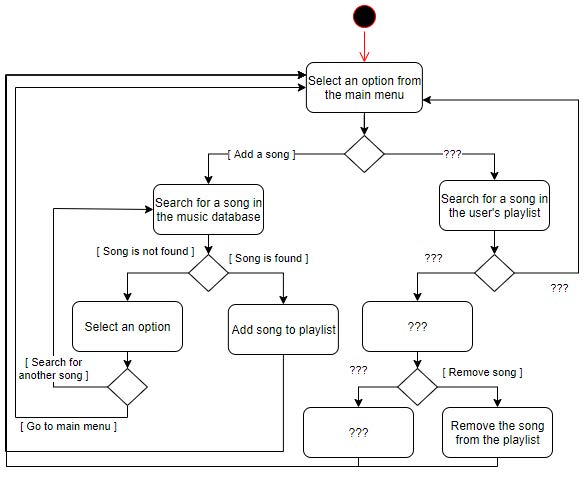
\includegraphics[scale=0.75]{Exercise 01_ Practice Problems.jpg}
    \end{center}

    \subsection*{Solution}

    \begin{center}
        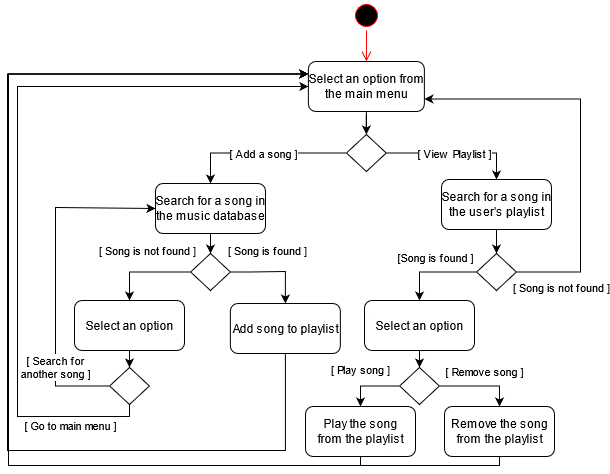
\includegraphics[scale=0.55]{Problem1.png}
    \end{center}


    %###################################################################################

    \section*{Problem 2}

    Below is a state diagram that models some of the states that the above system could go
    into. Fill in the six missing “???” parts.

    \begin{center}
        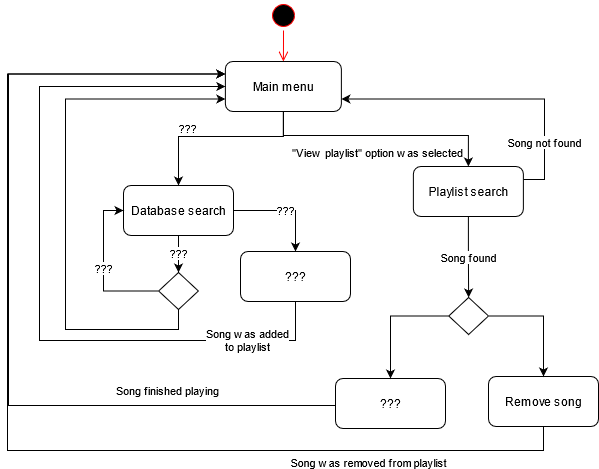
\includegraphics[scale=0.55]{Problem2_Example.png}
    \end{center}
    
    \subsection*{Solution}

    \begin{center}
        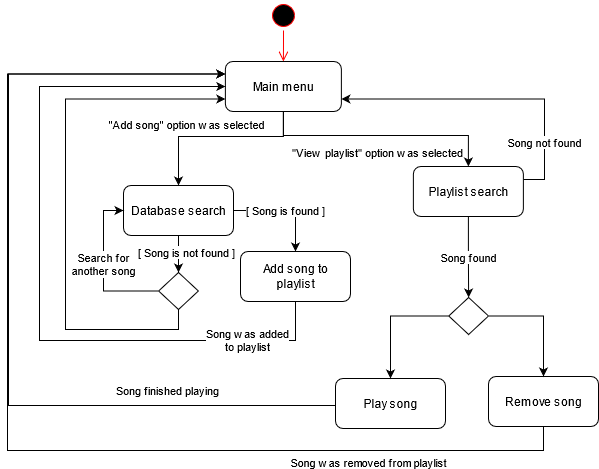
\includegraphics[scale=0.55]{Problem2.png}
    \end{center}


    %###################################################################################

    \section*{Problem 3}

    Let’s add a new option to the main menu of the online music playlist system, “Exit the
    system”.

    Modify the activity diagram from problem 1 to include a third option that the user can
    select from the main menu. If the user selects this new option, the system performs the
    actions to shut down and the activity diagram should end.

    \subsection*{Solution}

    \begin{center}
        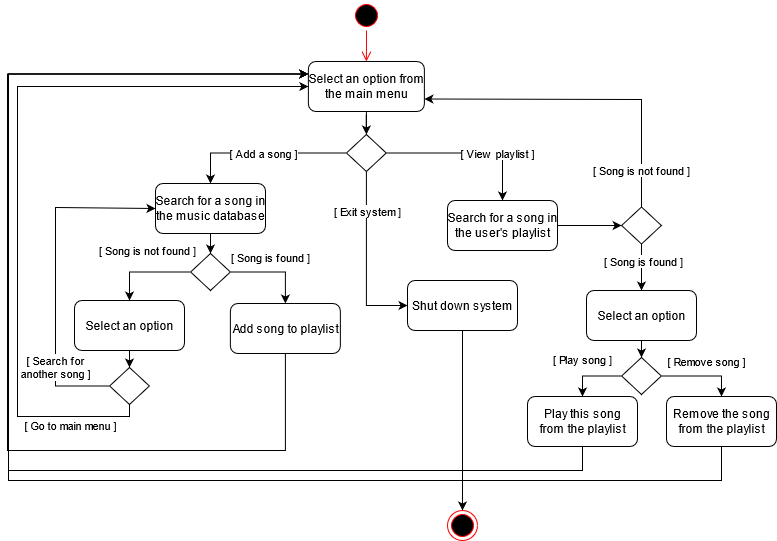
\includegraphics[scale=0.55]{Problem3.png}
    \end{center}


    %###################################################################################

    \section*{Problem 4}

    Let’s add a new option to the main menu of the online music playlist system, “Exit the
    system”.

    Modify the state diagram from problem 2 to include a state meant to indicate the system
    is shutting down. Once the system shut down is complete, the state diagram should end.

    \subsection*{Solution}

    \begin{center}
        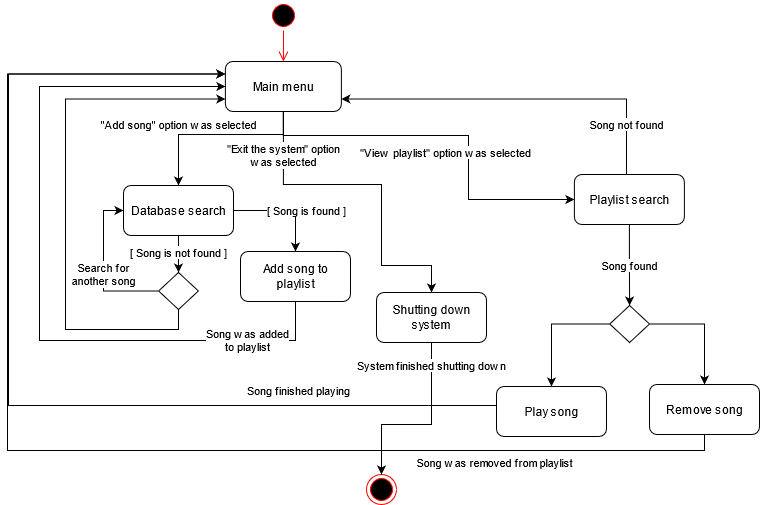
\includegraphics[scale=0.55]{Problem4.png}
    \end{center}


\end{document}